\documentclass[a4paper,12pt]{article}
\usepackage{float}
\usepackage[portuguese]{babel}
\usepackage[utf8]{inputenc}
\usepackage[T1]{fontenc}
\usepackage{graphicx}
\usepackage{hyperref}
\usepackage{titlesec}
\usepackage{longtable}
\usepackage{titlesec}
\usepackage{tabularx}

% Configuração para capítulos e seções
\titleformat{\section}{\large\bfseries}{\thesection}{1em}{}
\titleformat{\subsection}{\normalsize\bfseries}{\thesubsection}{1em}{}

\begin{document}

% Capa
\begin{titlepage}
    \centering
    {\Large UTFPR - UNIVERSIDADE TECNOLÓGICA FEDERAL DO PARANÁ} \\
    \vspace{0.5cm}
    {\large Bacharelado em Engenharia de Software - 6º Período} \\
    \vspace{1cm}
    {\bf DISCIPLINA: Oficina de Integração 1 - ES46F-ES61} \\
    \vspace{0.5cm}
    {\bf Professor: Eduardo Cotrin Teixeira} \\
    \vfill
    \rule{\linewidth}{1.5pt} \\
        \vspace{0.5cm} \
    {\Huge \textbf{Documento de Projeto de Software}} \\
    \rule{\linewidth}{1.5pt} \\
    \vspace{1cm}
    {\Large Nome do Projeto} \\
    \vfill
    {\large Luccas Philot Goncalves\\
            Yuri Garcia Yoshida\\
            João Marcos Ribeiro da Costa\\
            João Pedro Correia Leite Moreira\\
            Álison Christian Rebouças Vidal de Carvalho\\
            
    }
    \vspace{1cm}
    {\large Cornélio Procópio} \\
    {\large 2025} \\
\end{titlepage}


% Sumário
\tableofcontents
\newpage


\section{Introdução}
\subsection{Contexto}
O TEDI é um projeto de extensão da UTFPR - Campus Cornélio Procópio que promove a inclusão digital de idosos por meio de oficinas e cursos gratuitos. Criado em 2024, surgiu da necessidade de reduzir a exclusão tecnológica que afeta a terceira idade. Muitos idosos enfrentam dificuldades no uso de celulares, computadores e serviços online, e o projeto visa proporcionar autonomia e confiança no uso dessas tecnologias. O projeto oferece oficinas práticas, atividades lúdicas e cursos divididos em dois módulos: Informática Básica e Smartphones e Aplicativos, com foco em metodologias acessíveis ao público idoso.

\subsection{Justificativa}
A exclusão digital entre idosos é um problema que afeta sua autonomia, autoestima e inserção social. Muitos enfrentam dificuldades em tarefas cotidianas que envolvem tecnologia, como marcar consultas, acessar serviços bancários e se comunicar com familiares. Esse problema afeta diretamente os idosos e indiretamente seus familiares e cuidadores, criando uma barreira entre gerações. Com a implantação do projeto TEDI, espera-se promover um cenário em que os idosos possam utilizar a tecnologia com segurança e independência, facilitando sua inclusão digital e social.

\subsection{Proposta}
Com o intuito de apoiar o projeto TEDI, será desenvolvida uma aplicação que visa facilitar o acesso às informações do projeto de forma simples e acessível para todos os públicos, especialmente os idosos. A aplicação permitirá a visualização de notícias e informativos cadastrados pelos administradores do projeto, garantindo que os usuários estejam sempre atualizados sobre oficinas, cursos e demais atividades. Além disso, contará com uma página de formulário destinada ao cadastro de monitores voluntários, promovendo a ampliação da equipe de apoio. A interface será responsiva, acessível e projetada para uma navegação intuitiva, respeitando as diretrizes de acessibilidade.


\subsection{Organização do Documento}

Este documento está estruturado para apresentar de forma clara o desenvolvimento do projeto de software que apoiará o TEDI, iniciativa voltada à inclusão digital de idosos. O Capítulo 1 contextualiza o projeto, justifica sua importância social e tecnológica, e propõe a criação de uma aplicação web acessível. O Capítulo 2 descreve a solução proposta, detalhando seus objetivos, limitações, restrições e perfis dos usuários. O Capítulo 3 aborda o desenvolvimento do projeto, incluindo as tecnologias utilizadas, a metodologia adotada e o cronograma previsto. O Capítulo 4 trata dos requisitos do sistema, englobando requisitos funcionais e não-funcionais, além de diagramas de casos de uso e protótipos de telas que ilustram a interface da aplicação.

\newpage
\section{Descrição Geral do Sistema}
\subsection{Objetivos (Gerais e Específicos)}

Desenvolver uma aplicação web acessível, intuitiva e centrada no usuário idoso, com o intuito de divulgar e apoiar a administração do projeto TEDI, promovendo a inclusão digital e social.

\textbf{Objetivos Específicos}
\begin{itemize}
    \item Permitir a visualização clara e simplificada de informações sobre oficinas, cursos e demais atividades do TEDI;
    \item Disponibilizar atualizações, comunicados e notícias relacionadas ao projeto;
    \item Oferecer um formulário acessível para o cadastro de monitores voluntários;
    \item Garantir que a interface da aplicação atenda às diretrizes de acessibilidade digital, considerando as limitações do público idoso;
    \item Facilitar o gerenciamento de conteúdo por parte da equipe organizadora do projeto.
\end{itemize}

\subsection{Limites e Restrições}
A aplicação será desenvolvida exclusivamente para ambiente web, priorizando compatibilidade com os principais navegadores modernos. Inicialmente, não contará com funcionalidades como inscrição automática em cursos, interação entre usuários ou integração com redes sociais. A aplicação exigirá conexão com a internet e seguirá as diretrizes da WCAG 2.2, mas sua experiência pode variar conforme o dispositivo utilizado e o nível de familiaridade tecnológica do usuário.


\subsection{Descrição dos Usuários do Sistema}
O sistema será utilizado por diferentes perfis, cada um com objetivos e necessidades específicas:
\begin{itemize}
    \item \textbf{Alunos}: interessados em acompanhar notícias e informações gerais sobre o projeto;
    \item \textbf{Idosos}: público-alvo dos ofícios e cursos, acessam conteúdos de maneira simplificada e acessível;
    \item \textbf{Monitores}: voluntários que se cadastram para auxiliar nas atividades do TEDI;
    \item \textbf{Parceiros}: pessoas ou instituições que buscam informações para possíveis colaborações;
    \item \textbf{Equipe do Projeto}: responsáveis pela administração do conteúdo, cadastros e manutenção das informações exibidas.
\end{itemize}

\newpage
\section{Desenvolvimento do Projeto}

\subsection{Tecnologias e Ferramentas}

Para o desenvolvimento e implantação do sistema, serão utilizadas as seguintes tecnologias e ferramentas, organizadas conforme suas finalidades:

\begin{itemize}
    \item \textbf{Backend:} JavaScript, Express e PostgreSQL.
    \item \textbf{Frontend:} Angular com TypeScript.
    \item \textbf{Gerenciamento de Projeto:} Trello.
\end{itemize}

Essas tecnologias foram escolhidas por atenderem de forma eficiente às necessidades do projeto, possibilitando desenvolvimento ágil, integração entre as camadas do sistema e organização das tarefas.

\subsection{Metodologia de Desenvolvimento}

O modelo de desenvolvimento adotado será o \textbf{Kanban}. Esta metodologia foi escolhida por proporcionar flexibilidade na organização das tarefas, além de facilitar o acompanhamento do progresso individual e coletivo.\\

A aplicação do Kanban será estruturada da seguinte forma:

\begin{itemize}
    \item Será desenvolvido um protótipo inicial, que será apresentado e validado junto ao cliente.
    \item O fluxo de desenvolvimento será organizado em tarefas distribuídas no quadro do Kanban.
    \item As prioridades e os ajustes serão definidos em reuniões semanais com toda a equipe.
\end{itemize}

Essa abordagem permitirá uma evolução contínua do sistema, com entregas incrementais e foco em atender as necessidades do cliente de forma dinâmica.


\subsection{Cronograma previsto}
Definir o cronograma de desenvolvimento do projeto. Elaborar o cronograma por semana, definindo o responsável por cada tarefa. O cronograma deve contemplar todas as tarefas previstas no processo de desenvolvimento de software (descrito no item 3.2 Metodologia de desenvolvimento), conforme definido para o desenvolvimento do sistema.

\newpage
\section{Requisitos do Sistema}

\subsection{Requisitos Funcionais}

\begin{table}[H]
\centering
\label{tab:req-funcionais}
\begin{tabularx}{\textwidth}{|c|X|c|}
    \hline
    \textbf{Código} & \textbf{Descrição} & \textbf{Prioridade} \\
    \hline
    RF01 & O sistema deve permitir o cadastro de monitores com RA e CPF, impedindo duplicações. & Essencial \\
    \hline
    RF02 & O sistema deve permitir o login e logout do administrador. & Essencial \\
    \hline
    RF03 & O sistema deve permitir o gerenciamento de monitores (visualizar, editar e excluir). & Essencial \\
    \hline
    RF04 & O sistema deve disponibilizar um botão para copiar os e-mails dos monitores cadastrados. & Importante \\
    \hline
    RF05 & O sistema deve permitir o cadastro, edição e exclusão de notícias pelo administrador. & Essencial \\
    \hline
    RF06 & O sistema deve exibir uma página pública com o feed de notícias. & Essencial \\
    \hline
    RF07 & O sistema deve exibir na página inicial um carrossel com miniaturas das últimas notícias. & Desejável \\
    \hline
    RF08 & O sistema deve permitir aplicar filtros na página de notícias por data, palavra-chave e categoria. & Importante \\
    \hline
    RF09 & O sistema deve exibir uma página com informações sobre a equipe (foto, nome e função). & Desejável \\
    \hline
    RF10 & O sistema deve disponibilizar um formulário de contato que envia mensagens para o e-mail institucional do projeto. & Importante \\
    \hline
    RF11 & O sistema deve exibir uma barra de navegação fixa visível em todas as páginas. & Essencial \\
    \hline
\end{tabularx}
\caption{Requisitos Funcionais do Sistema}
\end{table}


\subsubsection*{Descrição dos Requisitos Funcionais}

\begin{itemize}
    \item \textbf{RF01 – Cadastro de Monitores:} O sistema deve permitir que alunos da UTFPR se cadastrem como monitores preenchendo um formulário com nome, RA, CPF e e-mail. O sistema deve validar RA e CPF para evitar duplicações.
    \item \textbf{RF02 – Login e Logout:} O sistema deve permitir que o administrador acesse as funcionalidades restritas com login e senha. O botão de logout deve estar visível nas páginas protegidas.
    \item \textbf{RF03 – Gerenciamento de Monitores:} O sistema deve exibir uma lista dos monitores cadastrados, permitindo que o administrador visualize, edite ou exclua os dados.
    \item \textbf{RF04 – Cópia de E-mails:} O sistema deve oferecer um botão para copiar os e-mails dos monitores já cadastrados, facilitando a comunicação por fora da plataforma.
    \item \textbf{RF05 – Gestão de Notícias:} O sistema deve permitir ao administrador publicar, editar e excluir notícias com título, corpo e imagens, com exibição automática no site.
    \item \textbf{RF06 – Feed de Notícias:} O sistema deve exibir uma página com o feed público de notícias, ordenadas por data, acessível a todos os visitantes.
    \item \textbf{RF07 – Carrossel de Notícias na Página Inicial:} O sistema deve exibir na página inicial um carrossel automático com miniaturas, título e imagem das últimas notícias.
    \item \textbf{RF08 – Filtro de Notícias:} O sistema deve permitir filtrar notícias por data, palavras-chave e categorias na página de notícias.
    \item \textbf{RF09 – Página da Equipe:} O sistema deve exibir uma página com nome, foto e função dos membros da equipe do projeto.
    \item \textbf{RF10 – Formulário de Contato:} O sistema deve disponibilizar uma página com formulário de contato, enviando as mensagens para o e-mail institucional do projeto.
    \item \textbf{RF11 – Barra de Navegação:} O sistema deve conter uma barra de navegação fixa no topo do site com acesso a todas as páginas.
\end{itemize}

\subsection{Requisitos Não Funcionais}

\begin{table}[H]
\centering

\label{tab:req-naofuncionais}
\begin{tabularx}{\textwidth}{|c|X|c|c|}
    \hline
    \textbf{Código} & \textbf{Descrição} & \textbf{Categoria} & \textbf{Prioridade} \\
    \hline
    RNF01 & O sistema deve ser responsivo, funcionando bem em dispositivos móveis e desktops. & Usabilidade & Essencial \\
    \hline
    RNF02 & O sistema deve ser hospedado em domínio e servidor da própria faculdade. & Ambiente & Essencial \\
    \hline
    RNF03 & O sistema deve ser compatível com navegadores modernos (Chrome, Firefox, Edge). & Compatibilidade & Importante \\
    \hline
    RNF04 & O sistema deve armazenar a senha do único administrador de forma criptografada. & Segurança & Essencial \\
    \hline
    RNF05 & O sistema deve implementar validações para evitar entradas inválidas e ataques como XSS e SQL Injection. & Segurança & Importante \\
    \hline
    RNF06 & O tempo de carregamento das páginas principais não deve ultrapassar 3 segundos. & Desempenho & Importante \\
    \hline
    RNF07 & O sistema deve seguir princípios de acessibilidade (como contraste, navegação por teclado e textos alternativos). & Usabilidade & Importante \\
    \hline
    RNF08 & O sistema deve utilizar ferramentas e bibliotecas gratuitas, compatíveis com o ambiente da faculdade. & Recursos & Essencial \\
    \hline
    RNF09 & O código do sistema deve ser organizado em camadas separadas: apresentação, lógica e dados. & Padronização & Desejável \\
    \hline
\end{tabularx}
\caption{Requisitos Não Funcionais do Sistema}
\end{table}

\clearpage

\subsection{Diagramas de Casos de Uso}

\begin{figure} [h]
    \centering
    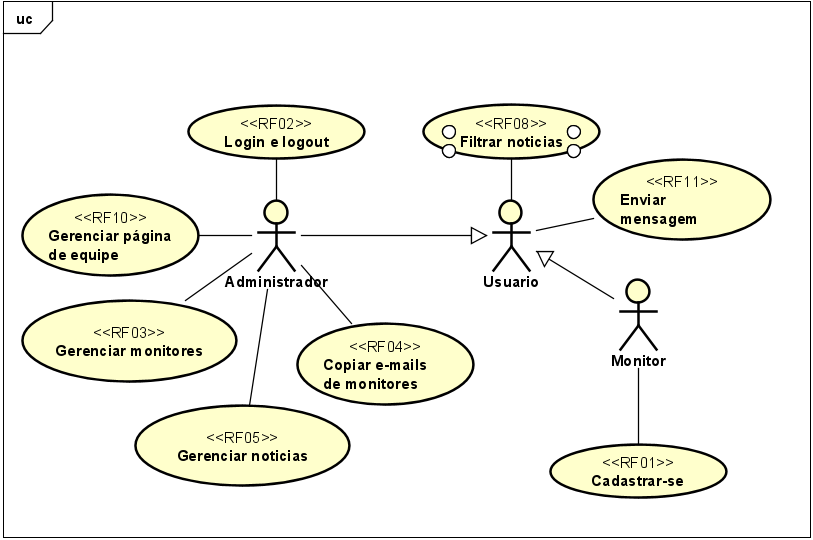
\includegraphics[width=1\linewidth]{caso_de_usoGeral.png}
    \caption{Caso de Uso Geral}
    \label{fig:enter-label}
\end{figure}

\subsection{Protótipos de Telas}
Apresentar o protótipo do sistema, que consiste na interface preliminar contendo um conjunto de funcionalidades e telas. 

\begin{figure}[h]
    \centering
    \includegraphics[width=0.7\textwidth]{prototipo.png}
    \caption{Protótipo da Tela de Login}
    \label{fig:prototipo_login}
\end{figure}

O protótipo é um recurso que deve ser adotado como estratégia para levantamento, detalhamento, validação de requisitos e modelagem de interface com o usuário (usabilidade).

As telas do sistema podem ser criadas na própria linguagem de desenvolvimento ou em qualquer outra ferramenta de desenho. Cada tela deve possuir uma descrição do seu funcionamento, constando pelo menos o objetivo da tela e dinâmica de navegação (de onde é chamada e que outras telas pode chamar). A descrição das telas deve registrar informações que possam ser consultadas para facilitar a implementação e a execução de testes, assim como a que requisitos funcionais se referem.

\newpage
\section{Análise do Sistema}
Este item deve apresentar a documentação da análise do sistema conforme o processo ou ciclo de vida descrito no capítulo 3. Organize o capítulo para apresentar os artefatos previstos e o que mais for necessário (protótipos, implementação, versões, telas, etc.), incluindo no mínimo (ajuste as subseções conforme necessário):

\subsection{Modelo do Banco de Dados}
Modelo Conceitual/Lógico: Apresentar o esquema relacional gráfico (opcionalmente pode ser apresentado também o Diagrama Entidade-Relacionamento) do banco de dados normalizado, constando as tabelas com os atributos e restrições (chaves).

Dicionário de dados: Apresentar o dicionário de dados do banco de dados. Documentar cada tabela com seus atributos mostrando nome do atributo, tipo, tamanho, descrição, se é obrigatório ou não, e o que mais for necessário para descrever os dados. Documentar também usuários, stored procedures, funções e qualquer outra implementação ligada ao banco de dados.

\subsection{Diagrama de Classes}
Apresentar o diagrama de classes previsto conforme a fase do projeto.

\subsection{Diagrama de Atividades}
Apresentar o diagrama de atividades, que representa o detalhamento de tarefas e o fluxo de uma atividade para outra de um sistema. Nem todas as tarefas do sistema necessitam de um detalhamento, portanto deve-se considerar no que o diagrama irá auxiliar na implementação do sistema para decidir quais atividades devem ser descritas.

\newpage
\section{Implementação}
\subsection{Descrição do código}
Descrever o sistema quanto ao código gerado. Explicar a organização dos arquivos, pacotes, classes ou quaisquer estruturas utilizadas no desenvolvimento do projeto, listando os componentes criados e sua estrutura. Use diagramas (Diagrama de Componentes, Diagrama de Pacotes) para ilustrar a implementação.

Descrever também convenções e padronizações para comentários no código, nomenclatura de classes, objetos, funções, etc. Se necessário, use exemplos.

\subsection{Implantação}
Explicar passo-a-passo para execução do software desenvolvido. Citar os requisitos necessários, configuração e providências para execução do projeto entregue. Se necessário, usar links, referências ou indicação dos recursos imprescindíveis para execução.

\subsection{Telas principais}
Apresentar as telas mais significativas do sistema, aquelas importantes para demonstração do seu funcionamento. Assim como nos protótipos, cada tela deve ser acompanhada de uma descrição sucinta de seu objetivo e sua dinâmica de navegação. O objetivo aqui é demonstrar o produto final.

\newpage
\section{Considerações Finais}
Apresentar e discutir os resultados obtidos e sua aplicabilidade. Abordar o que foi atingido e o que não foi, as limitações, possíveis integrações com outros projetos e continuação do sistema em trabalhos futuros.

\newpage
\section{Bibliografia}
\bibliography{}
Listar todas as referências utilizadas no projeto.


\end{document}
